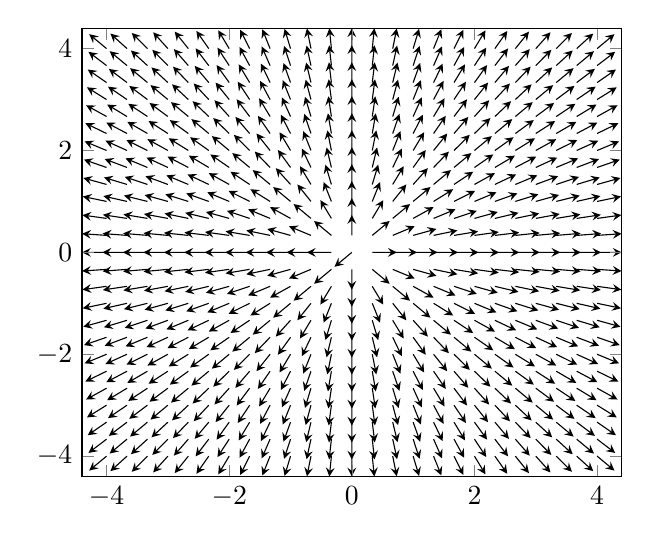
\begin{tikzpicture}
\begin{axis}[
    view = {0}{90}
]
    \addplot3[
        quiver = {
            u = {(x/(x^2+y^2))/sqrt((x/(x^2+y^2))^2+(-y/(x^2+y^2))^2)},
            v = {-(-y/(x^2+y^2))/sqrt((x/(x^2+y^2))^2+(-y/(x^2+y^2))^2)},
            scale arrows = 0.4,
        },
        -stealth,
        domain = -4:4,
        domain y = -4:4,
    ] {0};
\end{axis}
\end{tikzpicture}
\caption*{Representacion vectorial normalizada}